%
% experimente.tex
%
% (c) 2020 Prof Dr Andreas Müller, Hochschule Rapeprswil
%
\section{Fourier-Spektrum der Ableitung}
\rhead{Fourier-Spektrum der Ableitung}
\begin{figure}
\centering
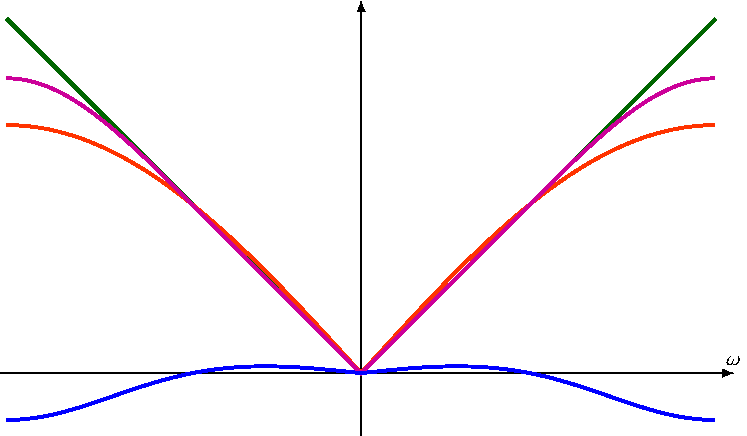
\includegraphics{papers/interdiff/experiment.pdf}
\caption{Fourier-Transformierte der Koeffizientenfolge für die Ableitung 
basierend auf dem Interpolationspolynom.
\label{interdiff:spektrum}}
\end{figure}
Die Fourier-Transformation der Ableitung einer Funktion ist
\[
\mathcal{F}
\frac{df}{dx}
=
i\omega\mathcal{F}f.
\]
\index{Fourier-Transformation}%
Dies gibt uns eine Möglichkeit, die Qualität der Ableitungsmethoden
von Abschnitt~\ref{section:interdiff:ableitung} zu messen.
Diese Berechnungsmethode ist eine Faltung mit der Folge der
Ableitungskoeffizienten.
Im Frequenzbereich wird daraus eine Multiplikation mit der
Fourier-Transformierten.
Der absolute Betrag der diskrete Fourier-Transformierten
der Ableitungskoeffizienten müsste also eine Betragsfunktion ergeben.

Die Resultate der Rechnung sind in Abbildung~\ref{interdiff:spektrum}
dargestellt.
Die Betragsfunktion ist grün dargestellt,
der gewöhnliche Differenzenquotient in hellrot.
Die pinke Kurve zeigt das Ableitungsverfahren, welches acht
Stützstellen verwendet.
Ganz offensichtlich wird dadurch das ideale Spektrum der
Ableitung besser approximiert.
Man kann allerdings auch erkennen, dass das Verfahren höhrer Ordnung
die hohen Frequenzen verstärkt, es ist also anfälliger auf Rauschen.



